\documentclass[a4paper,10pt]{article}
\usepackage[utf8]{inputenc}
\usepackage[english]{babel}
\usepackage{enumitem}	%enumerate
\usepackage{fancyhdr}	%intestazioni e piè pagina
\fancypagestyle{SE2}{% Software Engineering 2 Project Page Style
	\pagestyle{fancy}	
	%\fancyhead[LE,RO]{\slshape\rightmark}
	%\fancyhead[LO,RE]{\slshape\leftmark}
	%\fancyhead[L,R]{\slshape\rightmark}
	\cfoot{} % get rid of the page number 
	\fancyfoot[L]{\emph{PowerEnJoy}: \textbf{R}equirement \textbf{A}nalysis and \textbf{S}pecifications \textbf{D}ocument}
	\fancyfoot[R]{\thepage}
	\renewcommand{\headrulewidth}{0.4pt}
	\renewcommand{\footrulewidth}{0.4pt}
}
\pagestyle{SE2}
%\pagestyle{fancy}
\usepackage{graphicx}	%immagini
\usepackage[colorinlistoftodos]{todonotes}	%todo
%numeri romani maiuscoli
\newcommand{\RomanNumber}[1]{\uppercase\expandafter{\romannumeral #1\relax}}
\usepackage{hyperref} %link pdf
\hypersetup{
    colorlinks,
    citecolor=black,
    filecolor=black,
    linkcolor=black,
    urlcolor=black
}
\graphicspath{{./img/}} %extra root-path for images
\usepackage[T1]{fontenc}
%\usepackage[style=alphabetic]{biblatex}
%\usepackage[babel]{csquotes}
%\usepackage[bibstyle=authortitle,citestyle=verbose-trad1]{biblatex}
%\bibliography{RASD-main.bib}
%
\usepackage[toc,page]{appendix}
\begin{document}

\begin{titlepage}
\newcommand{\HRule}{\rule{\linewidth}{0.5mm}} % Defines a new command for the horizontal lines, change thickness here

\center % Center everything on the page
 
%----------------------------------------------------------------------------------------
%	HEADING SECTIONS
%----------------------------------------------------------------------------------------

\includegraphics[scale=0.3]{logo_poli.png}\\[0.5cm] % Include a department/university logo - this will require the graphicx package
\textsc{\LARGE Politecnico di Milano}\\[2cm] % Name of your university/college
\textsc{\Large Software Engineering \RomanNumber{2} project}\\[0.5cm] % Major heading such as course name
\textsc{\large \textbf{PowerEnJoy}}\\[1.5cm] % Minor heading such as course title

%----------------------------------------------------------------------------------------
%	TITLE SECTION
%----------------------------------------------------------------------------------------

\HRule \\[0.4cm]
{ \huge \bfseries Requirements Analysis\\ and Specifications Document}\\[0.4cm] % Title of your document
\HRule \\[1.5cm]
 
%----------------------------------------------------------------------------------------
%	AUTHORS SECTION
%----------------------------------------------------------------------------------------

\begin{minipage}{0.4\textwidth}
\begin{flushleft} \large
\emph{Authors:}\\
Davide \textsc{Piantella}\\
Mario \textsc{Scrocca}\\
Moreno R. \textsc{Vendra} % Your name
\end{flushleft}
\end{minipage}
~
\begin{minipage}{0.4\textwidth}
\begin{flushright} \large
\emph{Professor:} \\
Luca \textsc{Mottola} % Supervisor's Name
\end{flushright}
\end{minipage}\\[2cm]

% If you don't want a supervisor, uncomment the two lines below and remove the section above
%\Large \emph{Author:}\\
%John \textsc{Smith}\\[3cm] % Your name

%----------------------------------------------------------------------------------------
%	DATE SECTION
%----------------------------------------------------------------------------------------

{\large December 8, 2016}\\[0.5cm] % Date, change the \today to a set date if you want to be precise
{\large version 1.3}\\[2cm]
 
%----------------------------------------------------------------------------------------

\vfill % Fill the rest of the page with whitespace
\clearpage
\end{titlepage}


%----------------------------------------------------------------------------------------
%----------------------------------------------------------------------------------------
%----------------------------------------------------------------------------------------
%----------------------------------------------------------------------------------------
%	TABLE OF CONTENTS
%----------------------------------------------------------------------------------------
\pagenumbering{Roman}
\tableofcontents
%----------------------------------------------------------------------------------------
%	INTRODUCTION
%----------------------------------------------------------------------------------------
\clearpage
\pagenumbering{arabic}
\section{Introduction}
\subsection{Purpose of this document}
The purpose of a \textbf{R}equirement \textbf{A}nalysis and \textbf{S}pecifications \textbf{D}ocument is the process of discovering the purpose for which a software system was intended, by identifying stakeholders and their needs, and documenting these in a form that is amenable to analysis, communication, and subsequent implementation. \todo{Citation} It is also concerned with the relationship of software's factors such as goals, functions and constrains to precise specifications of software behavior, and to their evolution over time and across software families.

\subsection{Actual system}
The system we are to develop is brand new, there is no previous system.

\subsection{Scope}
PowerEnJoy is a car-sharing service that exclusively employs electric cars; we are going to develop a web-based software system that will provide the functionalities normally provided by car-sharing services, such as allowing the user to register to the system in order to access it, showing the cars available near a given location and allowing a user to reserve a car before picking it up.
A screen located inside the car will show in real time the ride amount of money to the user. When the user reaches a predefined safe area and exits the car, the system will stop charging the user and will lock the car. The system will provide information about charging station location where the car can be plugged after the ride and incentivize virtuous behaviours of the users with discounts.
	\subsubsection{Goals}
	\begin{enumerate}[label=\textbf{G\arabic*}]
		\item \label{goal:register} Allow users to register to the system
		\item \label{goal:login}Allow registered users to authenticate to the system
		\item \label{goal:position}Provide authenticated users with the position of available cars
		\item \label{goal:notifyMaintenance} Notify maintenance service with a list of not available cars 
		\item \label{goal:maintenanceDone} Provide the maintenance service with a way to notify the system when a car is available again 
		\item \label{goal:needMaintenance} Provide the user with a way to contact customer service to report a damaged car
		\item \label{goal:usersHistory} Provide a way to show to the user his rent and payment history and make these information accessible also to the customer service
		\item \label{goal:banUnbanUsers}Provide customer service with a way to ban users in order to prevent them from reserving or using other cars, and enable them to use the service again
		\item \label{goal:carReservation} Allow a user to reserve a car, if available, and hold that reservation for an hour
		\item \label{goal:reservationFee}Charge the user for 1\euro\ in case he hasn't used the car he reserved after an hour from such reservation
		\item \label{goal:completeRent}Allow a user to perform a complete rent: reserving a car, using it and leaving it terminating the rent, accomplishing the payment procedure related to aforementioned rent
		\item \label{goal:calculateCost}Calculate and charge the user for the correct amount of money he has to pay for his last ride, also considering the various discounts and fees applicable based on the ride
		\item \label{goal:moneySavingOption}Allow the user to enable a money saving option which provides him with a charging station as destination of the ride to get a discount on the cost of the aforementioned ride
	\end{enumerate}

\subsection{Glossary}
	\subsubsection{Definitions}
	\begin{description}
		\item[System:]the PowerEnJoy software we are to develop
		\item[Company:] the company we are developing the system for
		\item[Guest \emph{or} Guest user:] person who access the system as non logged user
		\item[Logged user \emph{or} Authenticated user:] authenticated person who is interfacing with the system
		\item[User:] \todo{only logged user? to be consistent with requirements} guest user or logged user
		\item[Banned user:] a user that can not use the system, he can only contact the customer care service
		\item[Registration:]  interaction between a non registered user and the system in which the user, providing all of the information required by the system for the creation of an account, receives from the system the credentials needed to authenticate to the system
		\item[Car:] an electric car owned by the company
		\item[Available car:] the car can be reserved by a user(i.d. the car is working correctly and its battery level is not critical)
		\item[Reserved car:] the car has been reserved by a user
		\item[In use car:] the user has ignited the car engine and he is still in the car
		\item[Not available car:] the car can not be reserved by a user (i.d. the car is not working correctly or its battery level is critical), a maintenance operator will deal with it
		\item[Battery level critical:] battery level under 20\%
		\item[Charging station:] location where cars owned by the company can be charged using a provided plug
		\item[Authentication \emph{or} Login:] interaction between guests and the system that grants authenticated user's privileges to a guest user
		\item[Safe area:] area of the map where a rent can be terminated without the corresponding additional fee
		\item[Payment procedure:] process which realizes the monetary transaction between the user and the system
		\item[Restricted access API:] API that can be used only by authorized person or system
		\item[GPS Coordinates:] GPS coordinates are a unique identifier of a precise geographic location on the earth
	\end{description}
\subsubsection{Acronyms}
	\begin{description}
		\item [RASD:] Requirements Analysis and Specification Document
		\item [API:] Application Programming Interface
		\item [GPS:] Global Position System
		\item [DBMS:] Data Base Management System
		\item [FSM:] Finite-State Machine
	\end{description}
\subsubsection{Abbreviations}
	\begin{description}
		\item [Km:] Kilometers
		\item [w.r.t.:] with respect to
		\item [i.d.:] id est
		\item [i.f.f.:] if and only if
		\item [e.g.:] exempli gratia
		\item [etc.:] et cetera
	\end{description}

\subsection{Document overview}
This document is structured in \todo{Complete, also with IEEE ref}
\begin{enumerate}
	\item \textbf{Introduction}: it provides an overview of this entire document and product goals
	\item \textbf{Overall description}: it describes general factors that affect the product providing the background for system requirements
	\item \textbf{Specific requirements}: it contains all system requirements
	\item \textbf{Use cases identification}: it contains the usage scenario of the system, the use case diagram and use cases description
	\item Appendix
\end{enumerate}

\begin{appendices}

	\section{Alloy model}
		\subsection{Source code}
		\lstinputlisting[language=alloy]{alloy/alloy2.0version.als}
		\begin{figure}[h!]
			\centering
			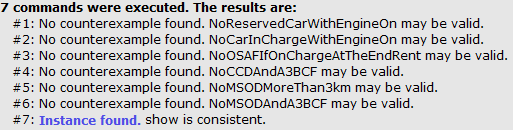
\includegraphics[]{alloy/AlloyResult.png}
			\caption{
				\label{fig:alloyExecutionResult} 
				Alloy execution result
			}
		\end{figure}
		\clearpage
		\subsection{Generated worlds}
			Note that in \autoref{fig:alloyWorld1} LoggedUser3 has been banned \emph{after} completing RentMade0.
			\begin{figure}[h!]
			\centering
			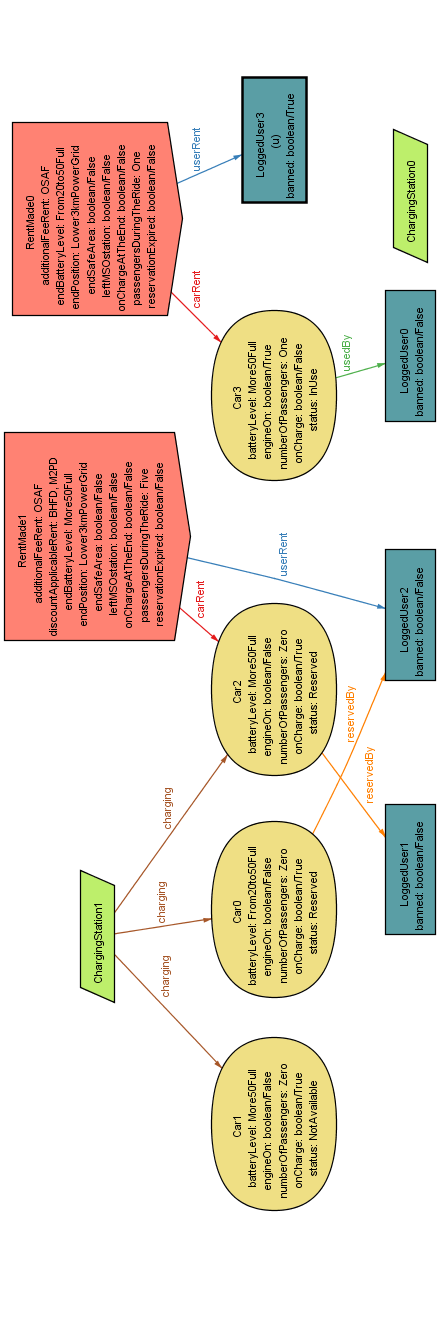
\includegraphics[scale=0.39]{alloy/AlloyWorld2.png}
			\caption{
				\label{fig:alloyWorld1} 
				First alloy generated world
			}
		\end{figure}
		\clearpage
		Note that in \autoref{fig:alloyWorld2} RentMade1 is actually a reservation expired of Car3 made by LoggedUser2. He now has reserved Car1.
		\begin{figure}[h!]
		\centering
		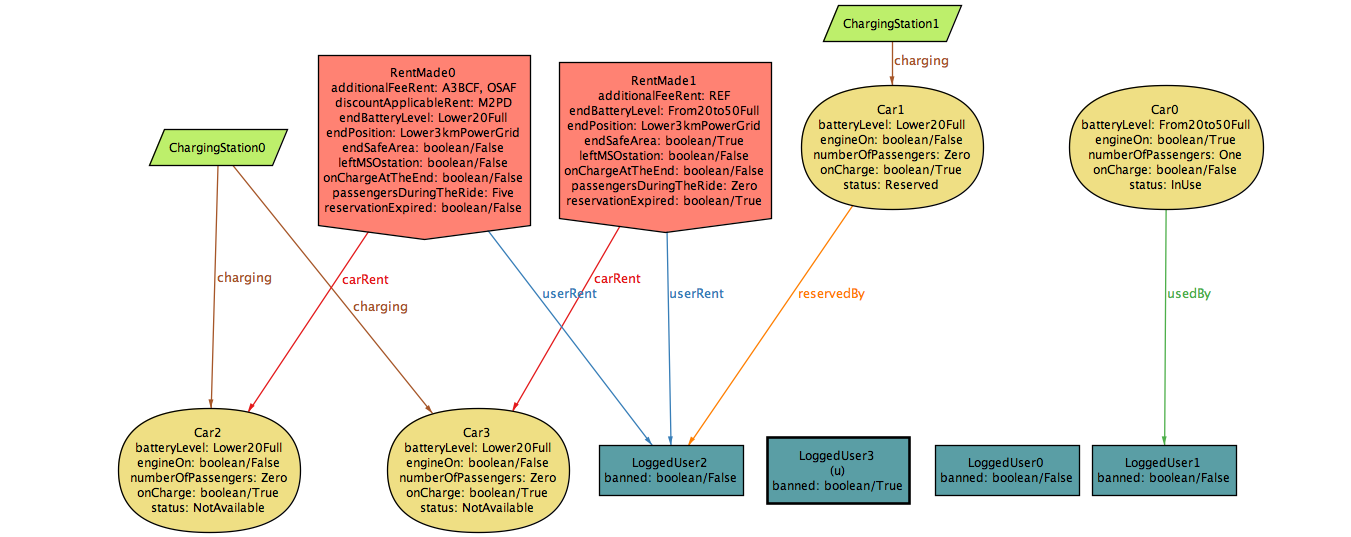
\includegraphics[scale=0.39]{alloy/AlloyWorld1.png}
		\caption{
			\label{fig:alloyWorld2} 
			Second alloy generated world
		}
		\end{figure}
		\clearpage
	\section{Software and tools used}
	For the development of this document we used
	\begin{itemize}
		\item \LaTeX{} as document preparation system
		\item Git \& \href{http://github.com}{GitHub} as version control system
		\item \href{http://draw.io}{Draw.io} for graphs
		\item StarUML for diagrams
		\item Alloy as model analyzer
	\end{itemize}
	
	\section{Hours of work}
	This is the team members' effort spent to redact this document:
	\begin{itemize}
		\item Davide Piantella: $\sim$ 48 hours
		\item Mario Scrocca: $\sim$ 48 hours
		\item Moreno R. Vendra: $\sim$ 45 hours
	\end{itemize}
\end{appendices}
\clearpage
\begin{thebibliography}{9}
\bibitem{RE}B. Nuseibeh, S. Easterbrook, \emph{Requirements Engineering: A Roadmap}, 2000
\bibitem{Zave}P. Zave, \emph{Classification of Research Efforts in Requirements
Engineering}, ACM Computing Surveys, 1997
\bibitem{Assignments} E. Di Nitto, L. Mottola, \emph{Assignments Software Engineering 2}, AA 2016-2017
\bibitem{IeeeRasd}IEEE Std 830:1993, \emph{IEEE Recommended Practice for Software Requirements Specifications}, 1993
\bibitem{WorldMachine}M. Jackson, \emph{The World and the Machine}, 1995
\bibitem{TextualAnalysis}R. J. Abbot, \emph{Textual (noun-verb) analysis},1983
\end{thebibliography}
\end{document}
